\documentclass[14pt,a4paper,titlepage]{article}
\usepackage[utf8]{inputenc}
%设置默认语言为德语
\usepackage[ngerman]{babel}
\usepackage{amsmath}
\usepackage{amsfonts}
\usepackage{amssymb}
\usepackage{graphicx}
\usepackage{titlesec}
%\usepackage{lipsum}
\usepackage{setspace}
%设置缩写格式
\usepackage[nohyperlinks, printonlyused, withpage]{acronym}
%设置取消拆分长单词
\usepackage[none]{hyphenat}
%设置对齐方式
\usepackage[document]{ragged2e}
%set sub figure
\usepackage{subcaption}
%设置超链接格式
\usepackage{hyperref}
\hypersetup{
	colorlinks=true,
	linkcolor=black,
	filecolor=blue,      
	urlcolor=black,
}

\urlstyle{same}
%设置各个分段的格式
\titleformat{\section}
{\normalfont\Large\bfseries}{\thesection}{1em}{}
\titleformat{\subsection}
{\normalfont\large\bfseries}{\thesubsection}{1em}{}
\titleformat{\subsubsection}
{\normalfont\normalsize\bfseries}{\thesubsubsection}{1em}{}
\titleformat{\paragraph}[runin]
{\normalfont\normalsize\bfseries}{\theparagraph}{1em}{}
\titleformat{\subparagraph}[runin]
{\normalfont\normalsize\bfseries}{\thesubparagraph}{1em}{}
%取消自动缩进
\setlength{\parindent}{0in}
%设置行间距
\linespread{1.213}
\spacing{1.213}
\begin{document}
	%self-made title page
	\begin{titlepage}
		\centering
		
\includegraphics[width=0.5\textwidth]{HSZG.png}\par\vspace{1cm}
		{\scshape\LARGE Hochschule Zittau/Görlitz \par}
		\vspace{1cm}
		{\scshape\Large Praktikumsbeleg\par}
		\vspace{1.5cm}
		{\huge\bfseries Untersuchung und Implementierung von Methoden der CAD-gestützten Roboterprogrammierung\par}
		\vspace{2cm}
		{\large\itshape Dongliang Cao\par}
		\vspace{2cm}
		\begin{minipage}{2.4in}
			{\large Bearbeitungszeitraum \\ Matrikelnummer \\ Betreuer der Ausbildungsfirma \\ Gutachter der Hochschule}
			
		\end{minipage}
		\hfill
		\begin{minipage}{2.0in}
			{\large 3 Monate \\ 
				217043 \\Dr.-Ing. habil. Fan Dai \\
			Prof. Dr. Stefan Bischoff}
		\end{minipage}
		% Bottom of the page
		\vfill
		{\large \today\par}
	\end{titlepage}

	\renewcommand{\abstractname}{Danksagung}

	\begin{abstract}
		
		Ich möchte mich bei Prof. Stefan Bischoff bedanken, dass er mein Betreuer an der Hochschule ist, und mich bei dem Praktikum unterstützt. 
		\bigbreak
		Ich möchte auch Dr. Dai Fan, meinem Betreuer im ABB Forschungszentrum danken. In meinem Praktikum hat er mir bezüglich theoretischer Fachkenntnisse und auch im praktischen Anwendungsbereich viel Unterstützung gegeben. Er hat mir alles eindeutig erklärt mit viel Geduld und Verständnis. 
	\end{abstract}
	\renewcommand{\abstractname}{Selbständigkeitserklärung}
	\begin{abstract}
		
		Ich versichere hiermit, dass ich meine Praxisarbeit mit dem Thema „Untersuchung und Implementierung von Methoden der CAD-gestützten Roboterprogrammierung“ selbstständig verfasst und keine anderen als die angegebenen Quellen und Hilfsmittel benutzt habe. Ich versichere zudem, dass die eingereichte elektronische Fassung mit der gedruckten Fassung übereinstimmt.
		\bigbreak
		Die Arbeit wurde bisher keiner anderen Prüfungsbehörde vorgelegt und auch noch nicht veröffentlicht.
		\vfill
		\begin{minipage}{2.0in}
			{\large \underline{Mannheim, \today}
			\\ Ort, Datum}
		\end{minipage}
		\hfill
		\begin{minipage}{2.0in}
			{\large \underline{\hspace{3cm}Dongliang Cao}
				\\ Unterschrift}
		\end{minipage}
	\end{abstract}
	\tableofcontents
	\pagebreak
	\section{Einleitung}
	\subsection{Problemstellung}
		Die zunehmende Komplexität von Produkten und Maschinen sowie kurze Produktionszyklen bei kleinen Losgrößen stellen die Industriebranche vor große Herausforderungen. Sowohl die Programmierung von Industrierobotern im Online-Modus mit Handbediengeräten als auch im Offline-Modus mit virtueller Simulation erfordert spezielle Kenntnisse in der Robotik und in fertigungsabhängigen Robotersteuerungssystemen. Bei komplizierten Aufgaben ist diese sehr zeitaufwändig. Insbesondere werden klein- und mittelständische Unternehmen mit zusätzlichen Hindernissen konfrontiert wie hohe Investitionen für die Ausbildung der nicht qualifizierten Mitarbeiter und die, wegen der Inbetriebnahme von Roboterzeller, verlängerten Produktionszyklen.   
	\subsection{Motivation}
		Um die Ingenieure von den wiederholenden, eintönigen und zeitaufwändigen Programmierverfahren zu befreien, damit sie sich mehr auf das Projekt selbst und dessen notwendigen Funktionen konzentrieren können, benötigt es neue Methoden für die Erzeugung des Roboterprogrammes, die effizienter, intuitiver und benutzerfreundlicher ist. 
		\bigbreak
		Grundsätzlich \ac{olp}, im Vergleich zur Online Programmierung kann dank der Simulationsumgebung mehr Zeit und Bemühung für den Benutzer sparen. Der Benutzter braucht nicht vor Ort den echten Roboter zu steuern, um die gewünschte Position zu erreichen, sondern am Bildschirm im Büro die notwendigen Positionen, Konfigurationen und Befehle in die Simulationsumgebung eingeben. Der Mangel an heutiger Offline-Software erklärt sich auch dadurch, dass, wenn der Benutzer eine lange Reihe von Bewegungsanweisungen definieren muss, er entweder viele Zeit benötigt, um jede Position zu definieren oder die genauen Positionen eventuell nicht bekannt sind. 
		\bigbreak
		Die meisten Informationen über die wichtigsten Positionen für die Bewegungsanweisungen beinhaltet normalerweise das Objekt, mit dem der Roboter interagiert. Die Informationen über das Objekt können durch die Analyse der notwendigen geometrischen Daten genutzt werden. Leider gibt es bisher wenige Ansätze für die Kombination von CAD-Daten und Offline Programmierung.
		\bigbreak
		Aus obigen Gründen möchte ich in meinem Praktikum ein Add-In-Programm in Robotstudio entwickeln, um die automatisch Erzeugung der nötigen Informationen für den Einschubprozess von zwei Objekten zu ermöglichen. 
		\begin{figure}[h!]
			\centering
			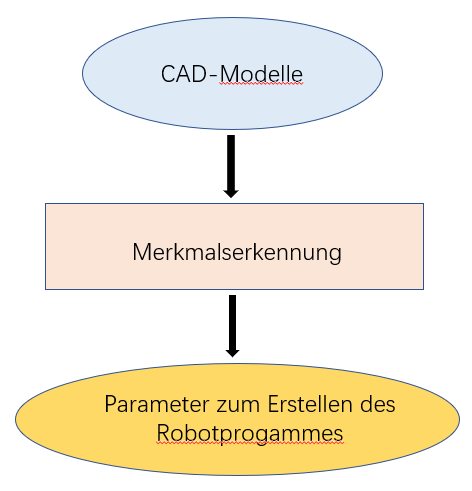
\includegraphics[width=0.5\textwidth]{Bearbeitungsverfahren.png}
			\caption{Bearbeitungsverfahren für CAD-Daten}
			\label{fig1}
		\end{figure}
	\subsection{Umsetzungsprozess}
	Die Realisierung des Prozesses beinhaltet:
	\paragraph{Extraktion und Analyse der Informationen einer CAD-Datei}
	
	Erwerb der geometrischen Informationen und Topologieinformationen des Objekts aus der CAD-Datei
	\paragraph{Filtern der Informationen einer CAD-Datei}

	Ausschluss der irrelevanten Informationen und Herausfiltern der Informationen, die Beziehungen zwischen Objekten enthalten
	
	\paragraph{Festlegung der Einschubrichutung und des Einschubabstandes}
	Kalkulation und Bestimmung der potentiellen Einschubrichtungen und entsprechenden -distanzen mithilfe von gefilterten geometrischen Informationen und Topologieinformationen  
	
	\paragraph{Visualisierung der Ergebnisse}
	Visualisierung der Ergebnisse in der Benutzeroberfläche von RobotStudio
	\pagebreak
	\section{Theoretische Grundlangen}
	\subsection{Offline Programmierung}
	\subsubsection{Definition}
	Die \acf{olp} ist eine Roboterprogrammierungsmethode, bei der das Roboterprogramm unabhängig von der eigentlichen Roboterzelle erstellt wird. Bei der Offline-Programmierung wird die Roboterzelle durch ein grafisches 3D-Modell in einem Simulator dargestellt. Heutzutage helfen OLP Roboterintegratoren dabei, die optimalen Programme für den Roboter zu erstellen, um eine bestimmte Aufgabe auszuführen. Bei der Simulation des Roboterprogramms können Roboterbewegungen, Erreichbarkeitsanalysen, Kollisions- und Beinahe-Erkennung sowie Zykluszeitberichte berücksichtigt werden\cite{offline-programming}.
	\bigbreak
	\paragraph*{Vorteile}
	\begin{itemize}
		\item [1)]
		Die Offline-Programmierung unterbricht die Produktion nicht, da das Programm für den Roboter außerhalb des Produktionsprozesses auf einem externen PC geschrieben wird.
		\item[2)]
		Integratoren und Endbenutzer können beim Entwurf einer Arbeitszelle Zeit und Geld sparen im Vergleich zur Online-Programmierung.
		\item[3)]
		Die Fähigkeit zu analysieren, wie sich eine Arbeitszelle verhält, bevor Zeit und Geld in Geräte investiert werden, sorgt für eine reibungslose Umsetzung vom Konzept zur Realität.
	\end{itemize}
	\paragraph{Vorgehensweise der \acl{olp}}
	\begin{itemize}
		\item[1)]
		\textbf{Erstellung der Arbeitszelle}
		\linebreak
		Eine Arbeitszelle bzw. Roboterzelle bezieht sich auf eine Kombination von einem oder mehreren Robotern und den damit verbundenen Werkzeugen, andere Werkstücke und Vorrichtungen. Wenn man eine Arbeitszelle erstellt, sollte man zuerst alle Komponenten in die Arbeitszelle importieren und danach platzieren. Außerdem muss der Roboter mit einer virtuellen Steuerung verbunden werden, um programmieren zu können.Ein Werkzeug ist ein spezielles Objekt (z.B. eine Lichtbogenschweißzange oder
		ein Greifer), das an einem Werkstück arbeitet. Für korrekte Bewegungen in
		Roboterprogrammen müssen die Parameter des Werkzeuges in den Werkzeugdaten
		angegeben werden. Der wesentliche Teil der Werkzeugdaten ist der \acf{tcp}.
		
		\item[2)] 
		\textbf{Programmierung von Robotern}
		\linebreak
		 Bevor der Benutzer ein Programm für seinen Roboter erstellt, sollte er die vorher genannte Arbeitszelle
		 einrichten, in der sein Roboter arbeiten soll, einschließlich des Roboters, der Werkzeuge
		 und Vorrichtungen.
		 \bigbreak
		 Das Verfahren für die Programmierung von Robotern kann in 5 Schritte unterteilt werden.
		 \begin{itemize}
		 	\item Erstellen von Positionen
		 	und Bahnen
		 	\item Prüfung der Positionsorientierung und Erreichbarkeit
		 	\item Synchronisieren des Programms
		 	mit der virtuellen
		 	Steuerung
		 	\item Ausführen von textbasierter
		 	Bearbeitung
		 	\item Kollisionserkennung
		 \end{itemize} 
	 	\item[3)]
	 	\textbf{Simulieren von Programmen}
	 	\linebreak
	 	Mit Simulationen werden vollständige Roboterprogramme auf einer virtuellen Steuerung ausgeführt. Durch Simulation kann die Zykluszeit berechnet, Kollisionen erkannt werden, die E/A-Signale simuliert und auch die Ereignisse (Aktion mit einem Trigger verbunden) behandelt werden, um festzustellen, ob das Robotersystem die Erwartung des Endbenutzers erfüllt.
	 	
	 	\item [4)]
	 	\textbf{Ladung des Programmes in die reale Steuerung}
	 	\linebreak
	 	Wenn die Simulation erfolgreich durchgeführt wurde, kann der Benutzer das automatisch generiert Programm von dem Computer in die Steuerung des realen Roboters laden.   
	\end{itemize}
	\subsubsection{Robotstudio}
	Robotstudio ist ein typisches Anwendungsbeispiel für die \acs{olp}, das von ABB entwickelt und unterstützt wird. RobotStudio ermöglicht dem Benutzer das Arbeiten mit einer Offline-Steuerung. Dabei
	handelt es sich um eine virtuelle IRC5-Steuerung, die lokal auf dem PC ausgeführt
	wird. RobotStudio basiert auf dem so genannten Virtual Controller, einer exakten Kopie der Originalsoftware, die den Roboter in Produktionsprozessen steuert. So sind realistische Simulationen möglich, denn zum Einsatz kommen die Daten und Konfigurationen, die auch in der realen Produktion zum Einsatz kommen\cite{robotstudio}.
	In meiner Arbeit, wird Robotstudio als eine Benutzeroberfläche zur Interaktion und Visualisierung von generierten Ergebnissen genutzt. Außerdem wird das Robotstudio \acf{sdk} als Programmbibliothek für die Entwicklung des Add-In-Programmes verwendet.
	\begin{figure}[h!]
		\centering
		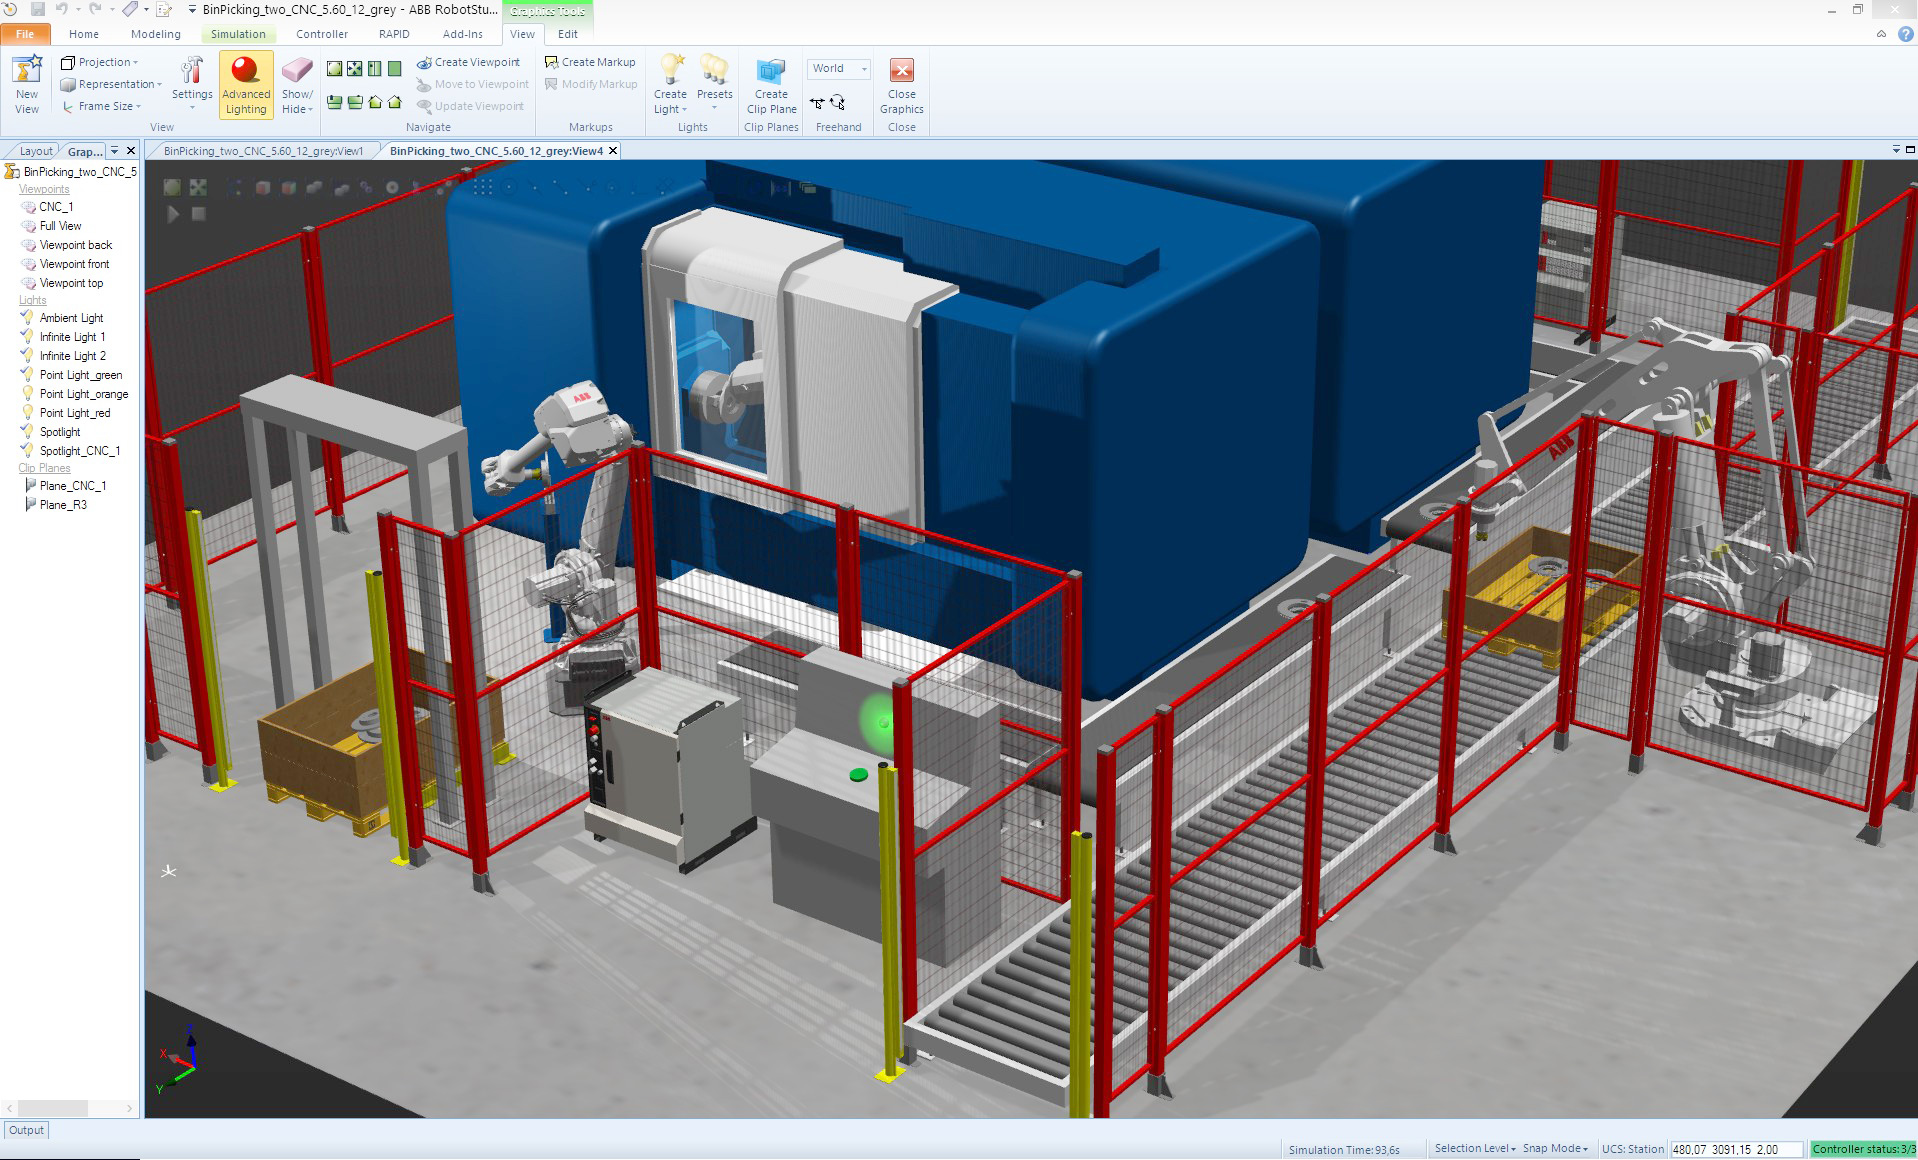
\includegraphics[width=0.8\textwidth]{robotstudio.jpg}
		\caption{Roboterzelle in Robotstudio}
		\label{fig2}
	\end{figure} 
	\pagebreak 
	\subsection{Geometrie und Topologie}
		Geometrie und Topologie sind die zwei wichtigsten Begriffe für die mathematische Darstellung der räumlichen Informationen von Objekten in der realen Welt. Die Geometrie bezieht sich in dieser Arbeit besonders auf die euklidische Geometrie, die sich mit Punkten, Geraden, Ebenen, Abständen und Winkeln beschäftigt, sowie den Begriffsbildungen und Methoden, die im Zuge einer systematischen und mathematischen Behandlung dieses Themas entwickelt wurden\cite{geometrie}. Neben der mathematischen Beschreibung der räumlichen Lage und Form von einzelnen Komponenten, beschreibt die Topologie die Lagebeziehung zwischen Geoobjekten, wie z.B. Knoten, Kanten und Maschen. In einfachen Systemen entsprechen Punkten, Knoten, Linien Kanten und Flächen Maschen\cite{topologie}.
		
		\bigbreak
		In den meisten CAD-Datei wird \acf{b-rep}, zu Deutsch „Begrenzungsflächenmodell“, als Modellierungsform eines Flächen- oder Volumenmodells verwendet. Ein typisches Beispiel ist eine Fläche wird als ein begrenzter Teil einer Oberfläche angesehen. Eine Kante ist ein begrenzter Teil einer Kurve und ein Scheitelpunkt liegt an einem Punkt. In der Welt des Datenaustauschs definiert \acf{step} auch einige Datenmodelle für \acs{b-rep}. Die allgemeinen generischen topologischen und geometrischen Modelle sind in der geometrischen und topologischen Darstellung nach ISO 10303-42 definiert\cite{b-rep}.
		    
	\subsubsection{Geometrie}
		Die Geometrie, die für die Modellierung von Geoobjekten in CAD-Systemen verwendet wird, ist die euklidische Geometrie. Die Geometrie kann man in vier Kategorien einteilen.
		\begin{itemize}
			\item[1)]
			\textbf{Punkte}, die in einem dreidimensionalen Raum existieren.
			\linebreak
			Der Punkt ist das grundlegendste geometrische Konzept in einem Raum. Ein Punkt im dreidimensionalen Raum wird normalerweise in einem kartesischen Koordinatensystem als eine Position dargestellt und die Position enthält drei Werte, die sich auf x, y, z-Koordinaten beziehen. 
			\bigbreak
			\emph{Hinweis:}
			\linebreak
			{\small Der Punkt in einem dreidimensionalen Raum kann nicht nur eine Position, sondern auch einen dreidimensionalen Vektor repräsentieren. Ein Vektor ist als eine räumliche Verschiebung von einer Position zu einer anderen Position zu definieren.}    
			\item[2)] 
			\textbf{Kurven}, die in einem dreidimensionalen Raum existieren.
			\linebreak
			In der Mathematik ist eine Kurve ein eindimensionales Objekt. Eindimensional bedeutet dabei informell, dass man sich auf der Kurve nur in einer Richtung (bzw. der Gegenrichtung) bewegen kann. Die Kurve können in der zweidimensionalen Ebene liegen(„ebene Kurve“) oder in einem höherdimensionalen Raum\cite{kurve}.
			\bigbreak
			In CAD-Systemen gibt es zwei wesentliche Arten vom Kurven: analytische Kurven und interpolierte Kurven.
			Alle analytischen Kurven werden von einem Parameter, der normalerweise t genannt wird, parametrisch dargestellt. Die drei wichtigsten Typen der analytischen Kurven sind Geraden, Ellipsen (einschließlich Kreise) und Helices.
			
			\begin{itemize}
				\item \emph{Geraden}
				\\
				Eine Gerade wird durch einen Punkt \(\vec{p_0}\) und eine Richtung \(\vec{r}\) dargestellt. Eine Gerade kann eine unendliche gerade Linie, eine teilweise begrenzte gerade Linie (ein Strahl) oder eine begrenzte gerade Linie (ein Liniensegment) darstellen
				
				\bigbreak
				
				Im dreidimensionalen Raum kann die Position eines Punktes auf einer Geraden durch die folgende parametrisierte Gleichung berechnet werden.
			    \[ \vec{p(t)} = \vec{p_0} + t\vec{r} \]
			    
				\item \emph{Ellipsen}
				\\
				Eine Ellipse wird durch einen Mittelpunkt \(\vec{p_0}\), einen Einheitsvektor \(\vec{n}\), der senkrecht zur Ebene der Ellipse ist, einen Vektor \(\vec{M}\), der die Hauptachse der Ellipse (einschließlich der Größe der Hauptachse) repräsentiert, und das Radiusverhältnis \(\alpha\) (das Verhältnis der Nebenachsenlänge zur Hauptachsenlänge) vollständig definiert.
				
				\bigbreak
				
				Im dreidimensionalen Raum kann die Position eines Punktes auf einer Ellipse durch die folgende parametrisierte Gleichungen berechnet werden.
				\begin{align*}
				\vec{p(t)} &= \vec{p_0} + \vec{M}\cos{t} + \vec{m}\sin{t}\\
			    \vec{m} &= \alpha(\vec{n}\times\vec{M})		
				\end{align*}
				\begin{figure}[h!]
					\centering
					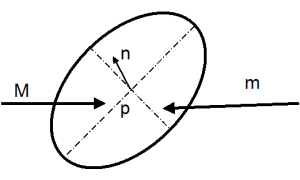
\includegraphics[width=0.5\linewidth]{ellipsen.png}
					\caption{Ellipse}
					\label{fig3}
				\end{figure}
				
				\item \emph{Helices}
				\\
				Eine Helix ist typischerweise eine dreidimensionale Spule, die wie ein Schraubengewinde auf der Oberfläche eines Zylinders liegt.
				Eine Helix wird definiert durch einen Wurzelpunkt, einen Einheitsvektor, der die Achse der Helix definiert, einen Vektor vom Wurzelpunkt zu einem Punkt auf der Kurve, die Steigung, die Drehrichtung und den Parameterbereich.
				
				\bigbreak
				
				Im dreidimensionalen Raum kann die Position eines Punktes auf einer Geraden durch die folgende parametrisierte Gleichung berechnet werden.
				\[ \vec{p(t)} = a\cos{t}\vec{x_0} + a\sin{t}\vec{y_0} + bt\vec{z_0}\]
				
				\begin{figure}[h!]
					\centering
					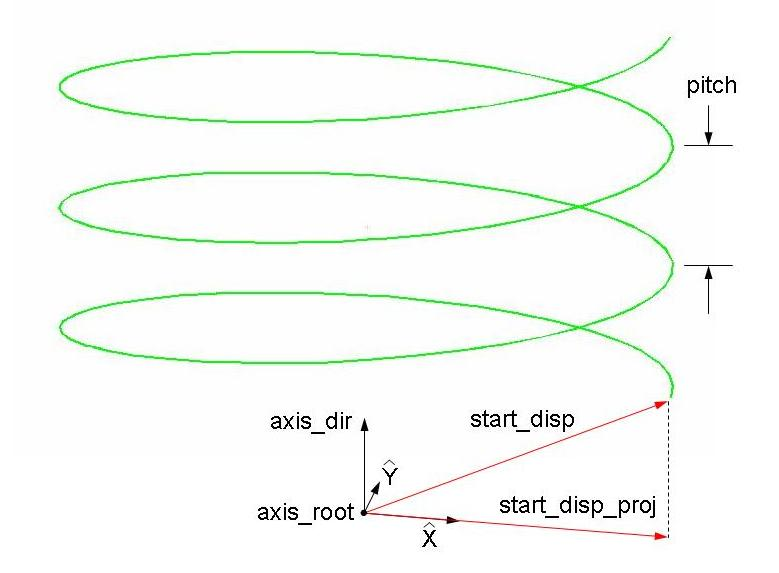
\includegraphics[width=0.4\linewidth]{helix.png}
					\caption{Helix}
					\label{fig4}
				\end{figure}
			\end{itemize}
			\item[3)]
			\textbf{Oberflächen}, die in einem dreidimensionalen Raum existieren.
			\\
			Der Begriff Oberfläche hat mehrere Bedeutungen. In CAD-Systemen wird dieser Begriff am häufigsten in seinem geometrischen oder mathematischen Sinne verwendet, um ein zweidimensionales Objekt in einem dreidimensionalen Raum mit einer einzigen geometrischen Definition zu beschreiben.
			\bigbreak
			
				Änlich wie bei Kurven, in CAD-System können Oberfläche im Wesentlichen in zwei Gruppen eingeteilt werden: analytische Oberflächen und interpolierte Oberflächen.
				Alle analytischen Oberflächen werden von zwei Parametern, die normalerweise u, v genannt werden, parametrisch dargestellt. Die vier wichtigsten Typen der analytischen Oberflächen sind Ebenen, Kegel, Kugel und Torus.
			
			\begin{itemize}
				\item \emph{Ebenen}
					\\
					In der Geometrie repräsentiert eine Ebene eine unendliche ebene Fläche oder einen begrenzten Bereich auf einer solchen Fläche.
					Die Parameter einer Ebene werden durch einen Punkt und einen Normalenvektor definiert. Die Parametrisierung einer Ebene wird durch zwei zusätzliche Parameter definiert: einen Vektor senkrecht zur Normalen, der die U- Parameterrichtung und Skalierung widerspiegelt, sowie eine Flag, die angibt, ob die Parametrisierung der Ebene für Rechts- oder Linkshänder erfolgt.
					
					\bigbreak
					Normalerweise wird eine Ebene in Bezug auf das rechtshändige Koordinatensystem definiert \( (\vec{U},\vec{V},\vec{N}) \).
					Die Richtung von \( \vec{U}\) ist von dem entsprechenden VeKtor bestimmt und die Richtung von \( \vec{V}\) ist durch \( (\vec{N}\times\vec{U}) \) bestimmt.
					
					\begin{equation*}
					\vec{p(u,v)} = \vec{R_0} + u\vec{U} + v\vec{V}
					\end{equation*}
					\begin{figure}[h!]
						\centering
						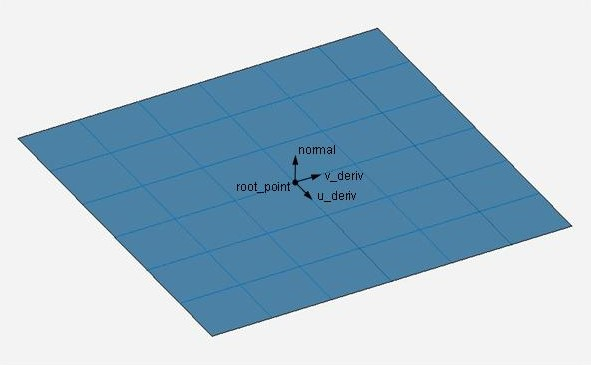
\includegraphics[width=0.5\linewidth]{plane.png}
						\caption{Ebene}
						\label{fig5}
					\end{figure}
				
				\item \emph{Kegel}
					\\
					In der Geometrie repräsentiert ein Kegel entweder einen Kegel oder einen Zylinder. Die Geometrie eines Kegels wird durch eine Basisellipse und den Sinus und Cosinus des Haupthalbwinkels des Kegels definiert. Die Normale der Basisellipse repräsentiert die Achse des Kegels. 

					\begin{align*}
						x &= au\cos{v}\\
						y &= au\sin{v}\\
						z &= u
					\end{align*}
					\begin{figure}[h!]
						\centering
						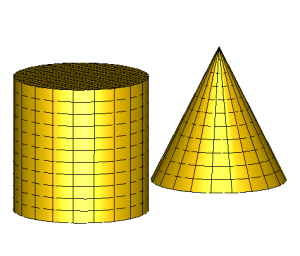
\includegraphics[width=0.5\linewidth]{cone.png}
						\caption{Kegel}
						\label{fig6}
					\end{figure}
				
				\item \emph{Kugel}
				\\
				In der Geometrie repräsentiert eine Kugel alle Punkte im dreidimensionalen Raum, die sich im Abstand R von einem festen Punkt dieses Raumes befinden. Der feste Punkt heißt der Mittelpunkt der Kugel und r ist eine reelle Zahl, die als Radius bezeichnet wird.
				\bigbreak
				Die parametrische Gleichung für eine Kugel lautet:	
				\begin{equation*}
					\vec{p(u,v)} = \vec{C} + |R|\sin{u}\vec{P} + |R|\cos{u}(\cos{v}\vec{Q} + \sin{v}\vec{R})
				\end{equation*}
				\(\vec{C}\) ist der Mittelpunkt der Kugel\\
				\(\vec{P}\) ist der Polrichtung\\
				\(\vec{Q}\) ist die Richtung zum Ursprung des Parameterraums\\
				\(\vec{R} = \vec{P}\times\vec{Q}\) 
					\begin{figure}[h!]
					\centering
					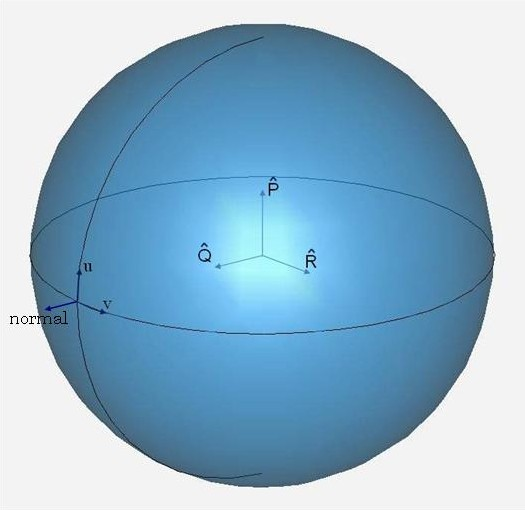
\includegraphics[width=0.5\linewidth]{kugel.png}
					\caption{Kugel}	
				\end{figure}
			\end{itemize}
		\end{itemize}
		\pagebreak
	\subsubsection{Topologie}
		Das Grundkonzept von \acf{b-rep} ist die Topologie, die beschreibt, wie Elemente begrenzt und verbunden werden. Topologie beschreibt die Beziehungen zwischen unterschiedlichen Geoobjekten.
		\bigbreak
		Durch Topologie kann, zum Beispiel, ausgedrückt werden, dass eine Kante \( E_1 \) durch die Eckpunkte  \( V_1 \) und \( V_2 \) begrenzt ist. Falls wir auch wissen, dass eine andere Kante \( E_2 \) durch die Eckpunkte \( V_2 \) und \( V_3 \) begrenzt ist, dann können wir ableiten, dass die Kanten \( E_1 \) und \( E_2 \) benachbart sind, weil \( V_2 \) beide Kanten begrenzt. 
				\begin{figure}[h!]
				\centering
				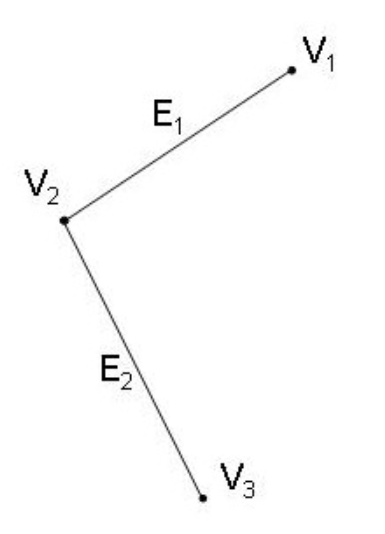
\includegraphics[width=0.25\linewidth]{beispieltopologie.png}
				\caption{Veranschaulichung des Topologie Beispiels}
				\label{fig9}
			\end{figure}
		\pagebreak
		\bigbreak
		Eine typische Hierarchie für topologischen Elemente mit Volumen besteht aus Körper, nicht verbundene Körper, Hüllen, Subhüllen, Flächen, Umrandungen, gerichtete Kanten, Kanten, Punkten. Für die Elemente ohne Volumen existieren keine Flächen, sondern Drähte.  
			\begin{figure}[h!]
			\centering
			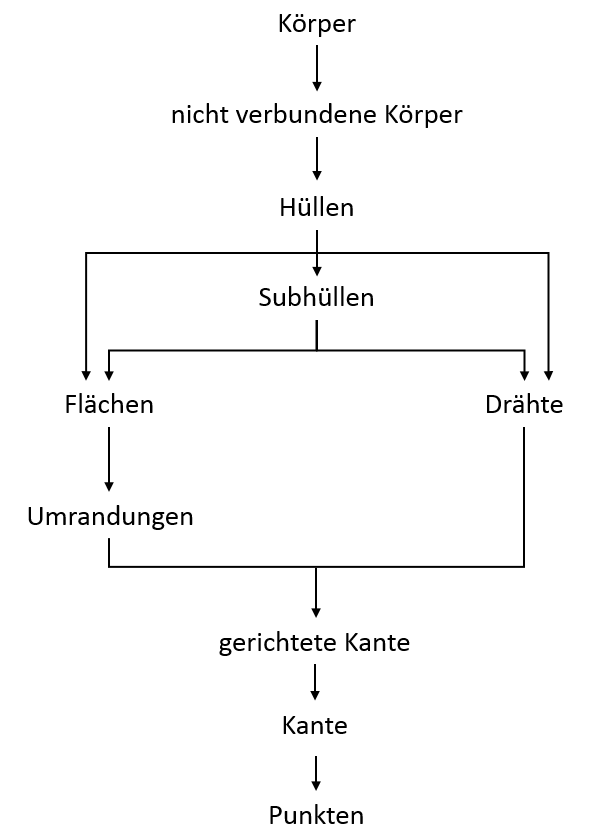
\includegraphics[width=0.7\linewidth]{topology.png}
			\caption{hierarchische Beziehungen zwischen topologischen Elementen}
			\label{fig8}
			\end{figure}
	\pagebreak
	\subsection{CAD Modellierung}
		Verschiedene CAD-Softwares unterstützen unterschiedliche CAD-Dateien. In SolidWorks werden beispielsweise ein Teil als ".prt" definiert, und eine Baugruppe als ".asm" gespeichert. Die verschiedenen proprietären CAD-Dateiformate werden von unterschiedlichen CAD-Konstruktionssoftwares wie Pro Engineer, SolidWorks und AutoCAD verwendet. Aufgrund der Vielfalt von CAD-Dateiformaten ist es sehr wichtig, ein neutrales CAD-Dateiformat, mit dem die Daten zwischen verschiedenen CAD-Programmen ausgetauscht werden können, zu finden.
		\begin{figure}[h!]
			\centering
			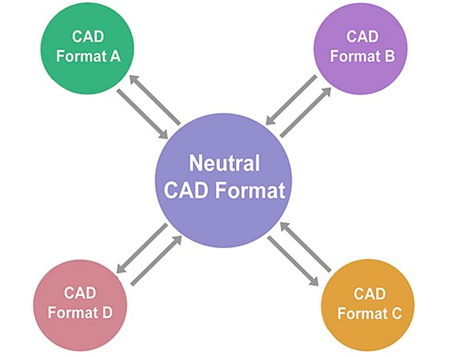
\includegraphics[width=0.5\linewidth]{cad.png}
			\caption{neutrales CAD-Dateiformat hilft Datenaustausch}
			\label{fig7}
		\end{figure}
		\break
		Eines der beliebtesten CAD-Dateiformat ist \acs{step}. Die Vorteile von \acs{step} spiegeln sich hauptsächlich in den folgenden vier Punkten wider.
		\begin{itemize}
			\item[1)]
			Ermöglicht das Anzeigen und Ändern von Geometrie mithilfe eines beliebigen CAD-Tools, das STEP-Geometrie interpretieren kann, und unterbricht die Abhängigkeit zwischen CAD-Systemen und Produktdefinition
			\item[2)] 
			Enthält das Assembly-Schema, das alle Connector-Entitäten enthält
			\item[3)] 
			Nützlich zum Gruppieren von mechanischen Elementen in Bestimmte Ansicht
			\item[4)] 
			Einfache Ableitung der impliziten Informationsinhalte. 
		\end{itemize}  
	\pagebreak
	\section{Aufgabenstellung}
		\subsection{Addin-Entwicklung in RobotStudio}
			Die Entwicklung für die Benutzeroberfläche zur Interaktion und Visualisierung wird mit dem RobotStudio SDK ausgeführt. Hierbei handelt es sich um ein Framework, mit dem die ABB RobotStudio Funktionen über die verfügbaren \ac{api} bearbeitet werden. Die Programmiersprache C\# wird zum Entwickeln der Front-End-Operationen verwendet. 
			Das SDK bietet Visual Studio-Projektvorlagen und APIs zum Erweitern von RobotStudio.
			\bigbreak
			\textbf{\emph{kurze Vorstellung für RobotStudio SDK und arbeitsrelevante Komponenten}}
			\\
			RobotStudio SDK wird unter das .NET Framework entwickelt und von C\# Programmiersprache geschrieben.  Grundsätzlich kann RobotStudio SDK nach unterschiedlichen Namespaces in verschiedenen Komponenten geteilt werden. Am häufigsten benutzte Namespaces sind:
			\begin{itemize}
				\item
				\textbf{ABB.Robotics.Math:}
				Der Namespace wie den Namen enthält alle Struktur und Klassen für mathematische Operationen in RobotStudio. Einige typische und häufig verwandte Beispiele sind Matrix4 zur Transformation (einschließlich Rotation und Translation), Vector3 zur Beschreibung einer Position, einer Vektor oder Eulersche Winkel und BoundingBox zur Beschreibung der minimale Begrenzungs- oder Umschließungsrahmen für eine Geometrie. 
				
				\item
				\textbf{ABB.Robotics.RobotStudio:}
				Der Namespace enthält Klassen, die die grundlegenden Bausteine der RobotStudio Pojektmodellen darstellen, z.B. das Speichern und Laden von Projekten, benutzerdefinierte Attribute, das Rückgängigmachen und verschiedene Maßeinheiten. Viele der Klassen in diesem Namespace werden als Basisklassen für die spezifischen Klassen im ABB.Robotics.RobotStudio.Stations-Namespace genutzt. Ein Beispiel davon ist ProjectObject, das als eine abstrakte Basisklasse für alle Objekte, die Teil eines Projekts sind, definiert wird.
				
				\item
				\textbf{ABB.Robotics.RobotStudio.Environment:}
				Der Namespace enthält Klassen für die Beschäftigung mit der RobotStudio-Benutzeroberfläche, z.B. die Buttons, Windows und Kontextmenüs.
				
				\item
				\textbf{ABB.Robotics.RobotStudio.Stations:}
				Der Namespace enthält Klassen, die das RobotStudio-Objektmodell, das Projektmodell, die Simulationslogik und den Informationsstrom darstellen. Die relevantesten Objektmodelle für meine Arbeit handelt es sich um die geometrische Topologie Klassen. Die Hierarchie für die Topologie kann durch folgende Abbildung eindeutig dargestellt wird. Die Klassen, die von der Basisklasse „GraphicComponent“ abgeleitet sind, kann direkt in \ac{gui} im RobotStudio hinzugefügt und gezeigt werden. Die anderen müssen eine Unterkomponente davon sein. 

				\begin{figure}[h!]
					\centering
					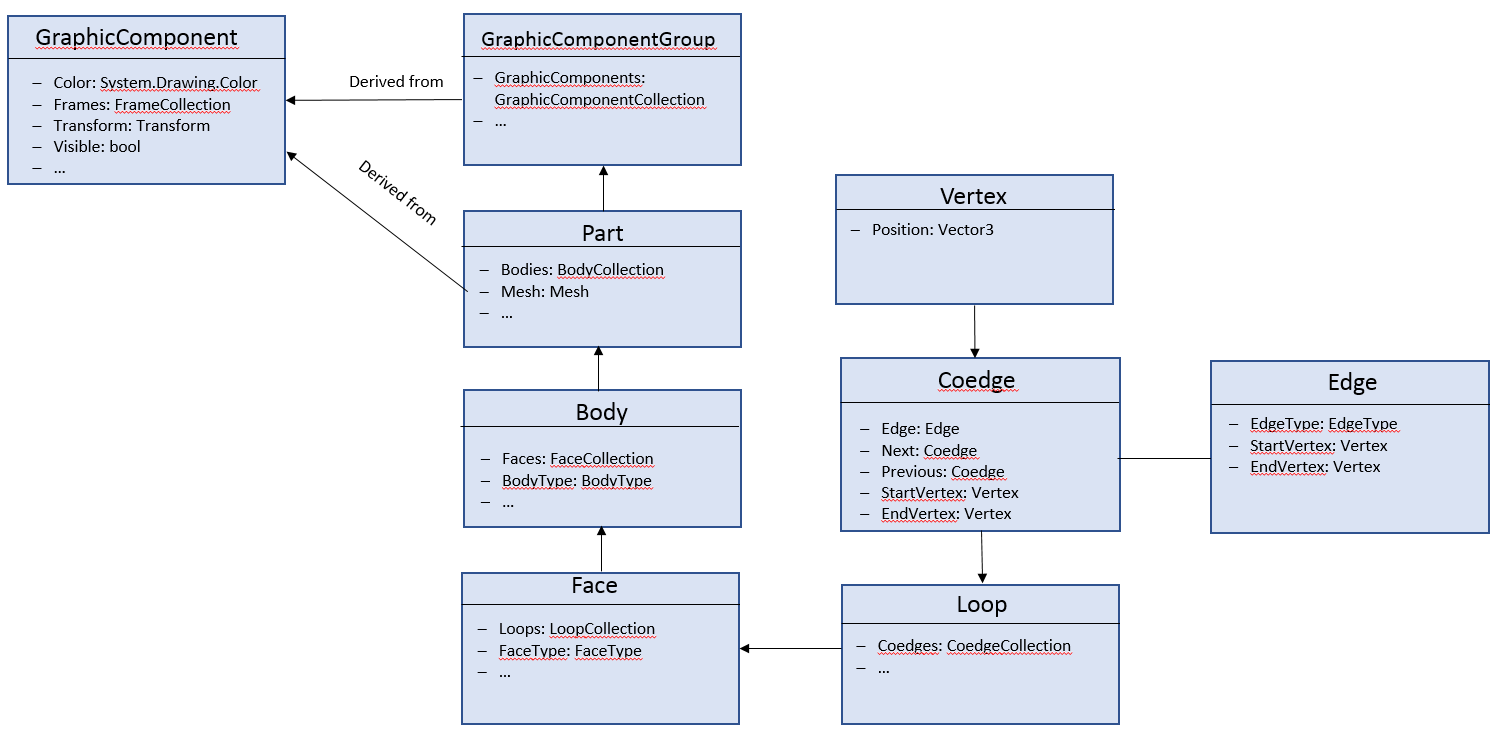
\includegraphics[width=0.8\linewidth]{TopologyRobotStudio.png}
					\caption{geometrische Topologie in RobotStudio}
				\end{figure}
				\item
				\textbf{ABB.Robotics.RobotStudio.Stations.Forms:}
				Der Namespace enthält Klassen für die Interaktion mit der 3D-Ansicht sowie eine Reihe von RobotStudio-spezifischen Kontrolle für Formulare und ToolWindows, z.B. Kontrolle für die Eingabe von Koordinaten und die Darstellung von Maßeinheiten.
			\end{itemize}
			\bigbreak
			
			\textbf{\emph{Die Vorgehensweise für die Entwicklung in RobotStudio}}
			\\
			\begin{itemize}
				\item[1)]
				\textbf{Herunterladen und Installation von RobotStudio SDK} 
				\\
				RobotStudio SDK kann man in die Website \href{http://developercenter.robotstudio.com/downloads_robotstudio}{ABB Developer Center} herunterladen. Bevor man RobotStudio SDK installiert, muss man beachten, dass zuvor Visual Studio 2015/2017 schon am Computer installiert ist. 
				
				\item[2)] 
				\textbf{Erstellung eines neuen Add-in Projektes in Visual Studio}
				\\
				Öffnen Sie zuerst Microsoft Visual Studio und wechseln Sie zu einem neuen Projekt. Aufgrund der Installation von RobotStudio SDK werden in der folgenden Abbildung die folgenden Vorlagen angezeigt.
				Wählen Sie aus der Liste RobotStudio 6.0 Empty Add-In aus und wählen Sie einen Namen für das Projekt.
					\begin{figure}[h!]
					\centering
					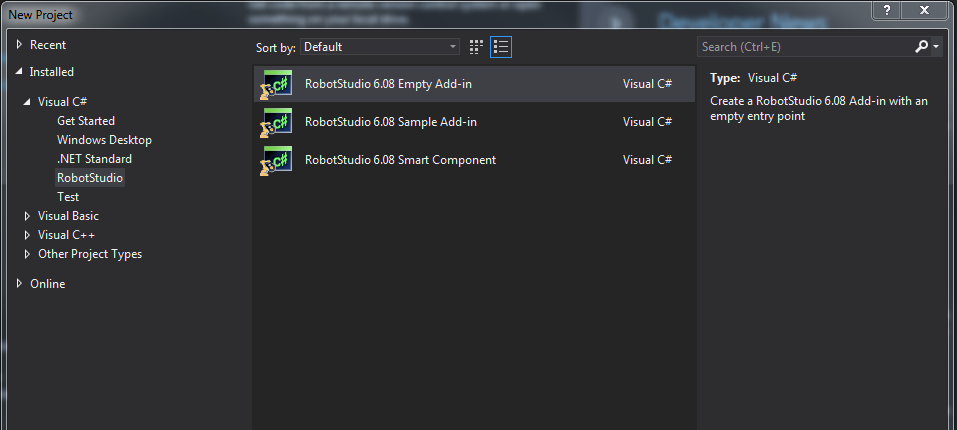
\includegraphics[width=0.8\linewidth]{addin.png}
					\caption{neues Projekt für RobotStudio Add-in auswählen}
					\end{figure}
				\bigbreak
				Aus dieser Vorlage wird die folgende Lösung mit der *.cs-Datei und den grundlegenden RobotStudio SDK *.dlls, die als Referenz zu dieser Lösung verwendet werden, generiert,. Außerdem wird mit der *.sln die Umgebung für die Entwicklung des RobotStudio-Add-Ins erstellt.
					\begin{figure}[h!]
					\centering
					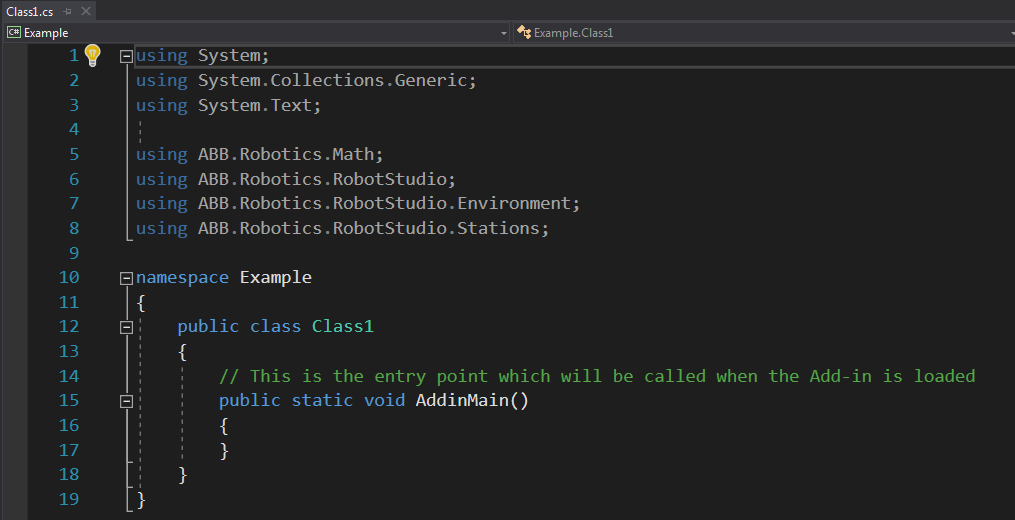
\includegraphics[width=0.8\linewidth]{cs.png}
					\caption{leere Lösung für RobotStudio Add-in}
					\end{figure}
				\bigbreak
				Führen Sie den Build-Befehl in Visual Studio aus, um den Code zu kompilieren und eine *.rsaddin-Datei für das Add-In zu generieren. Diese *.rsaddin-Datei ist dafür verantwortlich, dass RobotStudio die Add-In-Assembly (die .dll-Datei) laden kann.
				\item[3)]
				\textbf{UI-Entwicklung}
				\\
				Im RobotStudio-Arbeitsbereich gibt es verschiedene Arten von Bereichen, z.B. Ribbonbereich, Eigenschaftsbereich und Arbeitsbereich.\bigbreak
					\begin{figure}[h!]
						\centering
						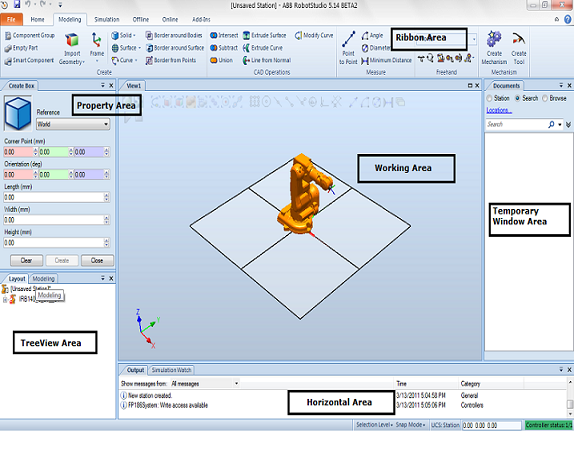
\includegraphics[width=0.6\linewidth]{workarea.png}
						\caption{Arbeitsbereich in RobotStudio}
					\end{figure}
				Um sich besser an die Gewohnheit des Benutzers anzupassen, verwende ich den Ribbonbereich und füge ich ein neues RibbonButton hinzu. 
				Die Reihenfolge für die Hinzufügung des Ribbons ist grundsätzlich wie folgendes:\\
					\begin{figure}[h!]
						\centering
						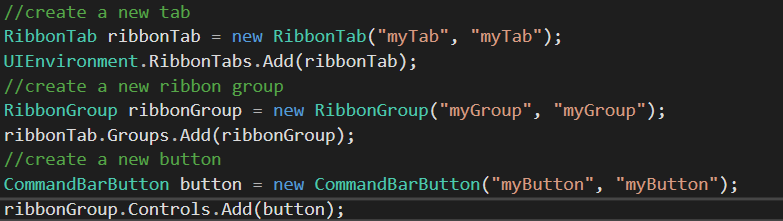
\includegraphics[width=0.8\linewidth]{createbutton.png}
						\caption{Der Kode für die Erstellung von einem Button}
					\end{figure}
				\pagebreak
				\emph{Erstens}, ein neues RibbonTab erstellen und in UIEnvironment hinzufügen.\\
				\emph{Zweitens},
				 ein neues RibbonGroup erstellen und in das vorher erstellte RibbonTab hinzufügen.\\
				\emph{Drittens},
				 ein neues RibbonButton erstellen und in das vorher erstellte RibbonGroup hinzufügen.
				\bigbreak
				Um die Organisation der Kodestruktur zu verbessern und später besser zu verwalten, habe ich für jeden individuellen Button eine neue Klasse erstellt, sodass die Funktionen und die Daten in dieselbe Klasse eingekapselt sind.
				\bigbreak  
				\begin{figure}[h!]
					\centering
					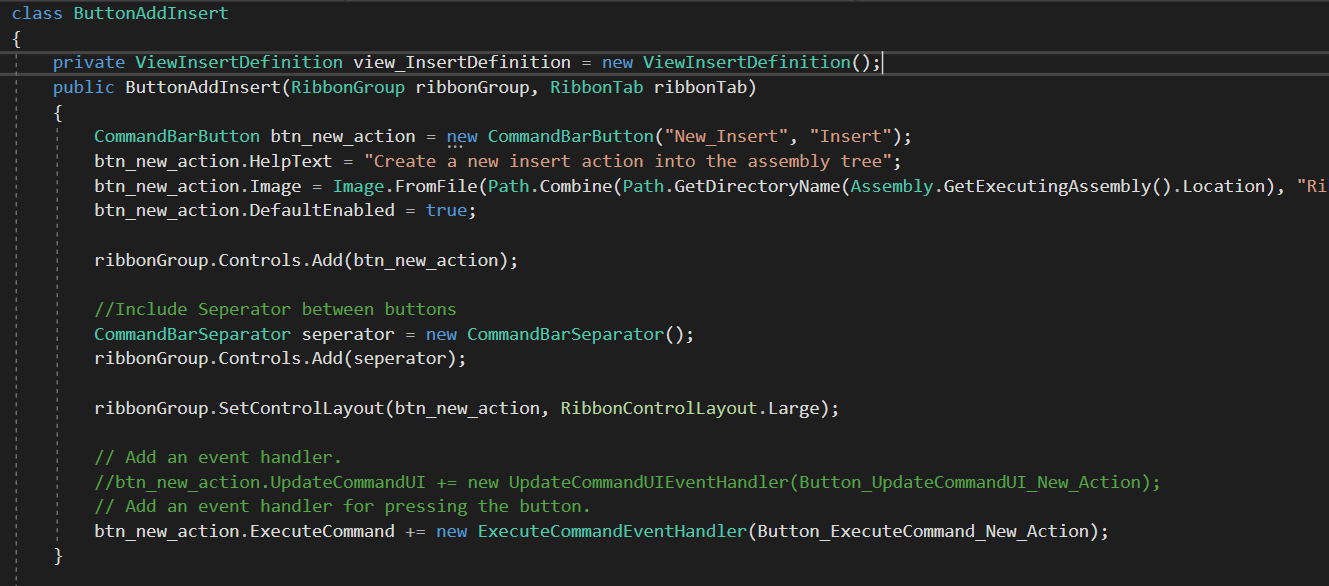
\includegraphics[width=0.8\linewidth]{buttonclass.png}
					\caption{Ein Beispiel für eine Buttonklasse}
				\end{figure}
				ToolWindow ist eine andere wichtige Klasse für \acs{gui}, die multifunktional als ein einziger Button ist. Ein ToolWindow ist ein Container für andere graphische Kontrolle, somit ist ein ToolWindow vielseitig und leicht erweiterbar.  Eine typische Anwendung für die Nutzung von ToolWindow ist wie folgende Abbildung gezeigt. \\
				\begin{figure}[h!]
					\centering
					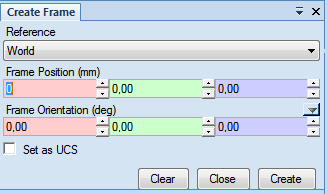
\includegraphics[width=0.8\linewidth]{toolwindow.png}
					\caption{Ein Beispiel für die Anwendung von ToolWindow}
				\end{figure}
				\pagebreak
				Das Beispiel wird zur Erzeugung eines neuen Frames genutzt. In diesem ToolWindow kann man unterschiedliche graphische Kontrolle sehen, wie ComboBox, Label, NumericTextBox, Button, die als ein Einheit zusammenarbeiten, um die Position und die Orientierung in Bezug auf unterschiedlichen Referenzframen zu bestimmen und endlich ein neues Frame zu erzeugen.
				\bigbreak
				In meinem kleinen Add-In-Programm, wählt der Benutzer einfach zwei Körper aus eine Geometrie Komponente und danach bestätigt, deshalb sieht das ToolWindow wie folgende Abbildung aus. \bigbreak
				\begin{figure}[h!]
					\centering
					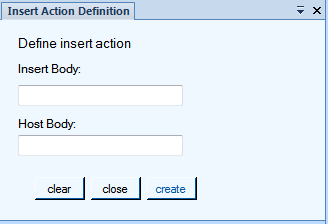
\includegraphics[width=0.8\linewidth]{inserttoolwindow.png}
					\caption{Tool Window für die Auswahl von zewi Körpern}
				\end{figure}
				\pagebreak
				Für die Auswahl von den gewünschten Körpern kann der Benutzer entweder in Bereich von Baumansicht oder in Arbeitsbereich durch Mausklick ermöglichen.  Um diese Funktion zu verwirklichen, muss man ein neues Ereignis „ObjetAdded“ unter dem Objekt „ProjectSelection“, das als eine Eigenschaft unter der Klasse „Selection“ ist, registrieren. Nach dem Kicken von „Create Button“ werde die Analyse von zwei ausgewählten Körpern beginnen und endlich die kalkulierte Einschubrichtung und -abstand zwischen zwei Körpern in Arbeitsbereich zeigen. 
				\begin{figure}[h!]
					\centering
					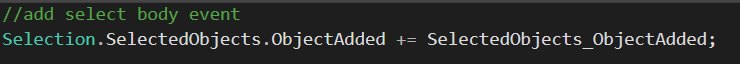
\includegraphics[width=0.6\linewidth]{ObjectAdded.png}
					\caption{Registrierung eines neuen Ereignisses}
				\end{figure}
				\begin{figure}[h!]
					\centering
					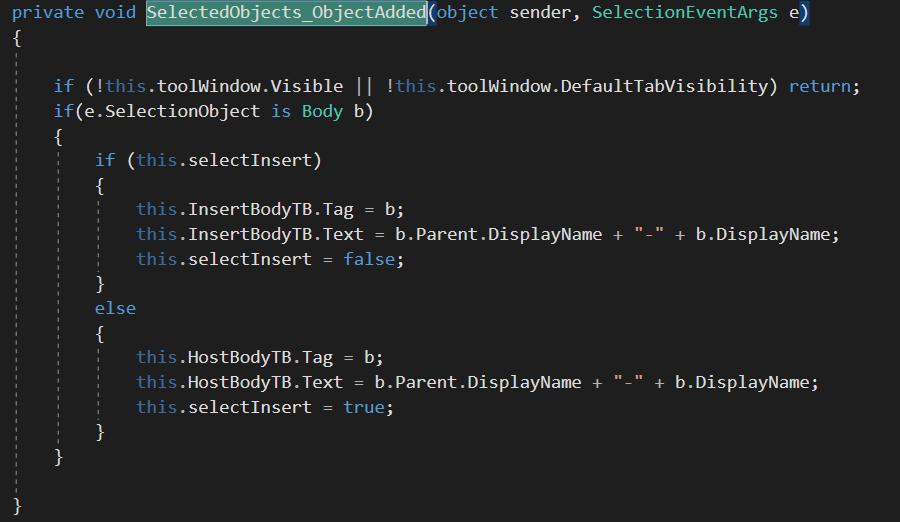
\includegraphics[width=0.6\linewidth]{ObjectAddedImplement.png}
					\caption{Inhalt des Ereignises}
				\end{figure}
			\end{itemize}
			\pagebreak
				
			
		\subsection{CAD-Modell Analyse Mithilfe von ACIS Modeler}
			\subsubsection{Kurze Vorstellung von ACIS Modeler}
			Der \ac{acis} ist eine objektorientierte dreidimensionale (3D) Geometrie- / Volumenmodellierungs-Engine von Spatial Corp. Sie dient als Grundlage jeder 3D-Modellierungsanwendung für Endbenutzer. ACIS wurde in C ++ geschrieben und bietet ein offenes Architektur-Framework für die Modellierung von Drahtmodellen, Oberflächen und Volumenkörpern aus einer gemeinsamen, einheitlichen Datenstruktur.
			\subsubsection{Vorstellung der angewandten Funktionen}
			Für meine Analyse werde ich wesentlich die Modellierungskomponente und die Komponente für die Analyse von Beziehung der Objekte benutzt. 
			\begin{itemize}
				\item 
				\textbf{Modellierungskomponent:}
				Die Modellierungskomponente lässt sich wesentlich als zwei Gruppe einteilen.
				\bigbreak
				 Die erste Gruppe beinhaltet alle Klassen und Strukturen, die für die Beschreibung und Modellierung der Geometrie und Topologie verantwortlich sind. Für die Topologie, die hierarchische Struktur von ACIS ist ähnlich wie die in obergenannte Struktur von RobotStudio nur ohne die oberen Klassen wie Part und GraphicComponentGroup, die als eine Visualisierungseinheit genutzt werden. Aber für die Geometrie, bietet ACIS andere separat geometrische Klassen an. Die Trennung von Geometrie und Topologie ermöglicht effizientere Algorithmen und bessere Modifikation von Geometrie. Jedes geometrische Objekt versteckt in ein topologisches Objekt, d.h. kann der Programme durch einen Pointer im topologischen Objekt das geometrische Objekt ergreifen. Zum Beispiel, das FACE ist ein topologisches Objekt in ACIS, das eine begrenzte Oberfläche repräsentiert, und dahinter verborgenes geometrisches Objekt SURFACE wird durch einen Pointer in FACE zugewiesen.
				 
				 Die zweite Gruppe beinhaltet viele nützliche \acs{api}, die hilfreich für die Traverse durch ganze topologische Hierarchie sind.  Die APIs vereinfacht die Arbeit von Programmen zu einem großen Teil. Zum Beispiel, wenn der Programme eine Operation für alle Ecken unter dem gleichen Körper durchführen möchte, muss er zuerst alle Ecken unter dem Körper bekommen, was sehr mühsam ist, weil der Programme zuerst alle Oberflächen, danach alle Schleife, endlich alle Kanten durchqueren muss. Glücklicherweise, bieten viele einfach Funktionen für solche Operationen auf unterschiedlichen topologischen Niveaus. 
				\pagebreak
				\item 
				\textbf{Komponente für die Analyse von Beziehung der Objekte}
				ACIS bietet verschiedene Mechanismen zum Analysieren der Objektbeziehung zwischen zwei Objekten. Es bietet allgemeine Funktionen für den Abstand von Objekte auf unterschiedlichen Niveaus, wie Körper und Körper, Körper und Fläche. Außerdem bietet es alternative Funktionen, die eine facettierte Annäherung an die Objekte verwenden, um den Mindestabstand zwischen ihnen zu bestimmen. Wenn weitere Informationen zu potenziellen Kollisionsbereichen benötigt werden, stellt ACIS eine Kollisionsfunktion bereit, um zu bestimmen, wie zwei Objekte interagieren. Darüber hinaus bietet ACIS eine Reihe von Funktionen, die die Einschlussbeziehung zwischen zwei Objekten oder zwischen einem Punkt und einem Objekt bestimmen.
				
			\end{itemize}
			\subsubsection{Die Verbindung zwischen RobotStudio und ACIS}
			Wie oben vorgestellt wird, RobotStudio SDK ist in C\# geschrieben und gleichzeitig ACIS ist in C++ geschrieben. Deshalb müssen wir eine Lösung finden, um in einer gemeinsamen .NET-Lösung die Funktionen zwischen diesen beiden Sprachen zu kommunizieren.
			\bigbreak
			Einer der beste Lösungen für die Kommunikation zwischen beiden Programmiersprachen ist, dank der Kompatibilität von .NET, die Anwendung von C++/\acs{cli}. Die \ac{cli} wird als eine von Microsoft entwickelte Variante der Programmiersprache C++ betrachtet, die den Zugriff auf die virtuelle Laufzeitumgebung der .NET-Plattform mit Hilfe von speziell darauf zugeschnittenen Spracherweiterungen ermöglicht.
			C++/CLI erfüllt die von Microsoft entwickelte Spezifikationen zur Sprach- und Plattform-neutralen Entwicklung und Ausführung von .NET-Anwendungen. Programme, die in C++/CLI geschrieben sind, können vom Compiler in \ac{cil} übersetzt und auf der virtuellen Maschine der .NET-Plattform betrieben werden\cite{cli}.
			\bigbreak
			Um sich die Referenzklassen in C\#, die automatisch von \ac{gc} verwaltet werden, und die Klassen in C++ voneinander zu unterscheiden, benutzt CLI eine andere Syntax für die Deklaration und Definition von den Referenzklassen in C\#. Ein typischer Unterschied ist wie folgende Abbildung gezeigt.
				\begin{figure}[h!]
				\centering
				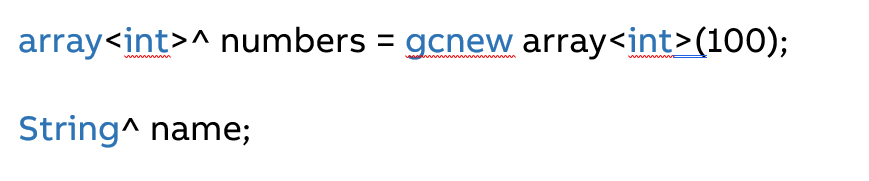
\includegraphics[width=0.5\linewidth]{cli.png}
				\caption{Deklaration von Array und String in CLI}
				\end{figure}
		
		\subsection{Einschubprozesserkennung}
		Wenn man über die Montage zwischen zwei Objekten nachdenkt, fällt ihm als Erstes die einfachste und gebräuchlichste Art von Montage ein, d.h. Einschub. Deshalb fokussiere ich in meine Praktikumsarbeit für den Einschub in einen Montageprozess. 
		\subsubsection{Definition des Einschubprozesses}
		Die erste Frage für die Analyse des Einschubprozesses ist wie kann man den Einschubprozess vollständig definieren, sodass der Prozess bei Generierung des Roboterprogrammes direkt benutzt werden kann.  Zur Verallgemeinerung und Vereinfachung des Prozesses kann man annehmen, dass der Einschubprozess ist nur von der Start-, Endposition und der Richtung abhängig.  Außerdem der Einschub ist auf eine lineare Translationsbewegung beschränkt und deshalb kann die Start- und Endposition durch einen Abstand ersetzt werden.    
		\begin{figure}[h!]
			\centering
			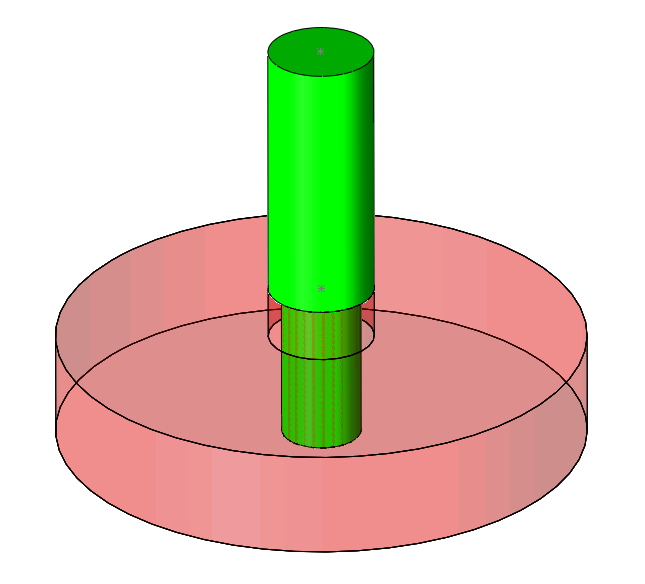
\includegraphics[width=0.5\linewidth]{Einschub.png}
			\caption{Ein Beispiel von Einschubprozess}
		\end{figure}
		\subsubsection{Definition des Modells in CAD}
		Die zweite Frage ist wie kann man das CAD-Modell, das relevante Objekte für den Einschubprozess beinhaltet, definieren. Wenn man den Einschubprozess einordnen möchte, ist die Anzahl der beteiligten Teile ein wichtiges Kriterium. Nach diesem Kriterium kann man den Prozess in zwei Arten teilen, nämlich eins-zu-eins und eins-zu-mehr.  
		\bigbreak
		Wenn wir eins-zu-mehr Baugruppe zerlegen, können wir feststellen, dass ein bewegliches Teil eine individuelle Montagebeziehung zwischen anderen Teilen in der Baugruppe hatte. Die Lösung für die mehrteilige Montage kann erreicht werden, indem ein bewegliches Teil entnommen und die Beziehung für jeden festen Teil nacheinander ermittelt wird. Dann können wir das einzelne Ergebnis zwischen einem beweglichen und einen festen Teil akkumulieren und den Montageprozess nacheinander durchführen. Gleichzeitig muss man beachten, dass die Reihenfolge eine wichtige Rolle spielt.\\
			\begin{figure}[h!]
			\centering
			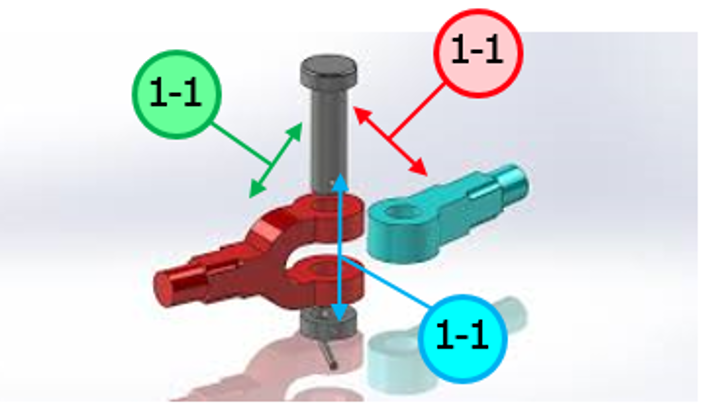
\includegraphics[width=0.5\linewidth]{eins-zu-mehr.png}
			\caption{Ein Beispiel für eins-zu-mehr Baugruppe}
			\end{figure}
		Aus obengenannten Gründen, können wir das Modell so definieren:
			\begin{itemize}
				\item Die Anzahl der Montageteile beträgt zwei
				\item Ein Montageteil gilt als fest und ein anderes als beweglich
				\item Anfangszustand von Montageteile ist montiert
			\end{itemize}
		\subsubsection{Die Lösung für Einschubrichtungserkennung}
			\paragraph{Die Grundidee}
			\begin{itemize}
				\item Die Auswahl von relevantesten Flächen in Festkörper und Einschubkörper separat.
				\item Extrahierung der möglichen Einschubrichtungen aus den ausgewählten Flächen.
				\item Festlegung der potentialsten Einschubrichtungen, indem der bewegliche Körper entlang der Richtung bewegen und eine Kollision zwischen beiden Körpern berechnen.
				\item Berechnung der Einschubdistanz aus die festgelegten Einschubrichtungen.
			\end{itemize}
			\paragraph{Die Auswahl von relevanten Flächen}
			spielt eine entscheidende Rolle für die Analyse von Einschubprozess zwischen zwei Objekten. Wenn zu wenig Flächen gefunden werden, kann die Fläche, die die Einschubrichtung enthält, vermissen. Wenn zu viel Flächen gefunden werden, ist die Effizienz der folgenden Analyse sehr niedrig. Deshlb kommt es zu dieser Frage, wie kann man die relevantesten Oberflächen definieren und herausfinden, sodass keine wichtigen Informationen für die Einschubrichtung übersehen werden, gleichzeitig keine überflüssigen Informationen enthalten sind.
			\begin{itemize}
				\item 
				\textbf{Entity Clash Calculations}
				\\
				Basierenden auf dieser Idee, habe ich zuerst die APIs für „Entity Clash Calculations“ benutzt. Die Eingänge für diese Funktion sind zwei Körper und die Ausgänge sind die zusammengestoßene Flächenpaare und deren Kollisionstypen. Die Vorteile für diese Funktion sind eindeutig. Auf diese Weise erhalte ich nicht nur die Kollisionsflächenpaare, sondern auch den Kollisionstyp, die sehr nützlich ist, um nicht verwandte Flächenpaare auszuschließen. Weil ich mich nur für die Flächenpaare interessiere, deren Normalvektoren einander entgegengesetzt sind.
				\begin{figure}[h!]
					\centering
					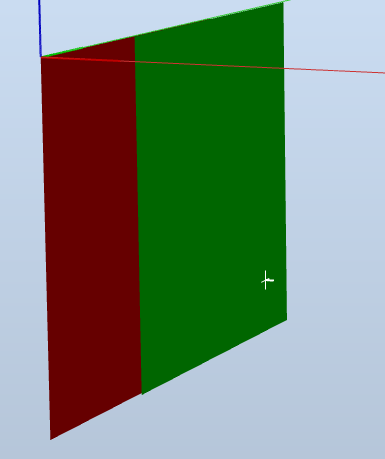
\includegraphics[width=0.5\linewidth]{facepair.png}
					\caption{Eine Flächenpaare mit entgegengesetzten Normalvektoren}
				\end{figure}
			
			
				 Trotz der Vorteile des Algorithmus habe ich bei Anwendung in verschiedenen CAD-Dateien festgestellt, dass, aufgrund der Toleranz- oder Abstandunterschied in Festkörper und Einschubkörper in unterschiedlichen CAD-Dateien, viele verwandte Flächen, die die Informationen über die Einschubrichtung enthalten, nicht herausgefunden werden können. Einer der wichtigsten Gründ in der Praxis für den Fehlschlag des „Entity Clash Calculations“ Algorithmus ist aufgrund der Präzision verschiedener CAD-Modelle der Mindestabstand bzw. der Grenzwert für die Bestimmung, ob zwei Körper zusammengestoßen sind, sehr unterschiedlich. Beispielsweise kann bei einer großen mechanischen Baugruppe der Mindestabstand zwischen Objekten einige Millimeter betragen, bei einem Präzisionsinstrument kann der Abstand zwischen Objekten jedoch nur einige Mikrometer betragen.
				 \pagebreak
				 
				 
				\item 
				\textbf{Entity Distance Calculation}
				\\ 
				Um obengenanntes Problem zu bewältigen, muss man den Mindestabstand in unterschiedlichen CAD-Modellen berücksichtigen. Deshalb habe ich stattdessen die APIs für „Entity Distance Calculation“ benutzt. Die verwandten Flächen nach diesem Kriterium sind die Flächen, die sich innerhalb der vordefinierten Entfernung von den anderen Körpern befinden. 
				\bigbreak
				Mit diesen Funktionen kann man nach der Genauigkeit von unterschiedlichen CAD-Modellen den Grenzwert selbst einstellen und die entsprechenden Flächen herausfinden. Gleichzeitig sollen die Nachteile des Algorithmus nicht übersehen werden. Einerseits, haben die Informationen zur Flächenpaaren und Kollisionstypen auf diese Weise verloren. Andererseits, gehören dazu viele nicht verwandte Flächen, von denen sich nur eine Kante oder ein Punkt im Mindestabstand befindet und keine Informationen für den Einschubprozess beinhalten. 
					\begin{figure}[h!]
					\centering
					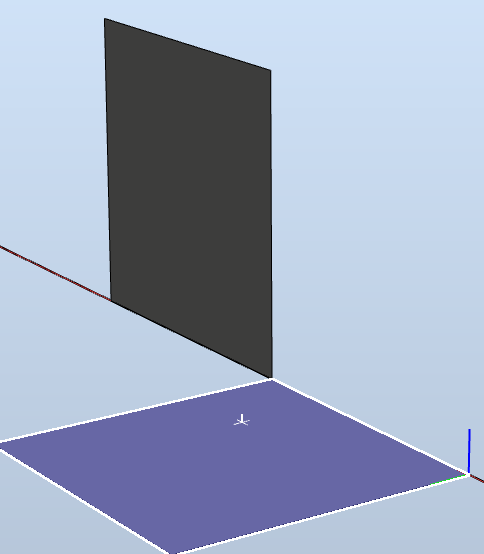
\includegraphics[width=0.3\linewidth]{faces.png}
					\caption{Nur ein Punkt von Flächen innerhalb des Abstandes}
				\end{figure} 
				\pagebreak
				\item 
				\textbf{Die Kombination von zwei Lösungen} 
				\\
				Die beiden Algorithmen haben ihre eigenen Vorteile und Nachteile, deshalb habe ich eine Kombination von diesen zwei Algorithmen versucht. 
				\begin{itemize}
					\item \textbf{Erster Schritt:}
					Mit der Entfernungsberechnung werden alle Flächen von Festkörper und Einschubkörper getrennt innerhalb des vordefinierten Mindestabstandes ausgewählt
					\item \textbf{Zweiter Schritt:}
					Lassen sich die Flächen verbleiben, die in einem anderen Körper eine entsprechende Fläche finden können, die sich innerhalb des Abstandes befindet und deren Normalvektor in entgegengesetzte Richtung weisen.
				\end{itemize} 
			
				  Durch die Kombination von zwei Lösungen reduziert die Anzahl der ausgewählten Flächen dramatisch und die nicht relevante Flächen werden ausgeschlossen.     
			\end{itemize}
		
		\paragraph{Extrahierung der möglichen Einschubrichtungen} 
			Um die potenziellen Einschubrichtungen von den ausgewählten Flächen extrahieren zu können, muss man zuerst festlegen, welche geometrische Informationen von einer Fläche der möglichen Einschubrichtung entsprechen. Nach der Analyse von unterschiedlichen Situationen kann ich annehmen, dass in den meisten Fällen die Einschubrichtung immer identisch mit einer der folgenden Richtungen ist:
			\begin{itemize}
				\item Die Richtung einer Kante auf einer Seitenfläche
				\item Die Richtung der Normalvektor auf Unterseite, falls es existiert
				\item Das Kreuzprodukt zweier Normalenvektoren, die nicht gegeneinader sind, auf zwei verschiedenen Seitenflächen. 
			\end{itemize} 
			Die nächste Aufgabe ist die Einordnung der ausgewählten Flächen. Am Anfang habe ich die Flächen in zwei Gruppen eingeteilt und das Einteilungskriterium ist ob eine einseitige Verlängerung des Normalvektors von der Flächemitte den Körper berührt. Aus der Gruppe, die den Körper nicht berührt, können wir die Richtung nach außen durch Summation ihrer Normalenvektoren bestimmen. Danach habe ich alle folgende Analyse in den anderen Gruppen durchgeführt, weil die Seitenflächen, deren Kante der Einschubrichtung entsprechen, befinden sich am meisten in der zweiten Gruppe. 
			\bigbreak
			  Erstens, habe ich die Geometrie berücksichtigt. Wenn die dahinter liegende Geometrie einer Fläche ein Kegel ist, können wir annehmen, dass die Achse des Kegels eine der möglichen Einschubrichtungen ist.
			  Wenn die ausgewählten Flächen in der zweiten Gruppe mindestens zwei Seitenflächen enthalten, die sich nicht gegenüberliegen, können wir davon ausgehen, dass das Kreuzprodukt ihrer Normalenvektoren eine der möglichen Einschubrichtungen ist. Außerdem wenn die einseitige Verlängerung einer Kante in der Seitenfläche den Körper nicht berührt, können wir auch annehmen, dass die Richtung der Kante eine der möglichen Einschubrichtungen ist. Alle mögliche Richtungen werden gespeichert und für den näschsten Schritt verwendet.
			  
		\paragraph{Festlegung der potentialsten Einschubrichtung}
		Nach der Suche nach der möglichen Einschubrichtungen muss ich auch entweder die Anzahl der Einschubrichtungen einschränken oder die möglichste Einschubrichtung herausfinden. Eine intuitive Lösung dafür ist „Entity-Entity-Clash“. Die Grundidee besteht darin, wenn der Einschubkörper entlang der Einschubrichtung herausgezogen werden kann, muss es in jede beliebige Position keine Kollision gibt.   
		\bigbreak
		Das Problem ist wie kann man den Abstand der Schiebung des Einschubkörpers für den Kollisionstest festlegen. Egal der Abstand zu groß oder zu klein ist, wird der Test fehlgeschlagen, d.h. keine Kollision existiert aber falsche Richtung. Die endliche Lösung läutert wie folgendes:
		\begin{itemize}
			\item Aus den endgültig ausgewählten Flächen im Fest- und Einschubkörper kann ich zwei Begrenzungsrahmen bestimmen und lassen sich die zwei Begrenzungsrahmen schneiden, um einen kleineren Begrenzungsrahmen zu erhalten.
			
			\item Festlegung der Bewegungsdistanz, indem die Entfernung entlang der Richtung innerhalb des Begrenzungsrahmens berechnen und mit einem Faktor wie 0.5 multiplizieren.
		\end{itemize}                                  
		Wenn entlang der Richtung keine Kollision gibt, kann die Richtung als einer der möglichsten Einschubrichtungen betrachtet wird. 
		
		\paragraph{Berechnung der Einschubdistanz}
		 Die Einschubdistanz muss gewährleisten, dass bei Anfangsposition von Einschubprozess keine Kollision zwischen beiden Körpern existiert. 
		 Von diesem Gedanken kann ich ausgehen, dass die Minimumeinschubdistanz zwischen Festkörper und Einschubkörper ist die Subtraktion von Maximaltiefe in Einschubkörper und Minimaltiefe in Festkörper entlang Einschubrichtung.\\
		 	\begin{figure}[h!]
		 	\centering
		 	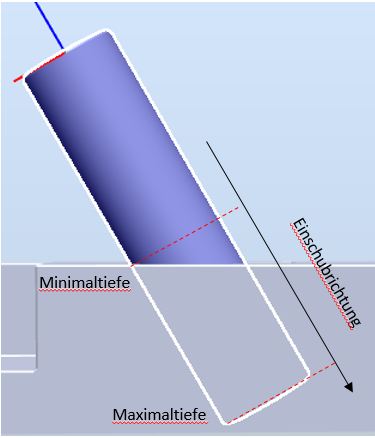
\includegraphics[width=0.3\linewidth]{Einschubdistanz.png}
		 	\caption{Ein Beispiel für die Berechung der Einschubdistanz}
		 	\end{figure} 
	 	
	 	Der Algorithmus für die Berechnung ist in diesem Fall ziemlich eindeutig und einfach.
	 		\begin{itemize}
	 			\item Finden alle Eckpunkte in ausgewählten Flächen in beiden Körpern
	 			\item Projektieren alle Eckpunkte in die Einschubrichtung und Finden die Maximaltiefe für Einschubkörper und Minimaltiefe für Festkörper
	 			\item \(Einschubdistanz = Maximaltiefe - Minimaltiefe\)
	 		\end{itemize}
	\section{Ergebnis und Diskussion}
		\paragraph{Geltungsbereich}
		Nach der Implementierung von dem obengenannten Algorithmus in unterschiedlichen CAD-Modellen, kann ich den Geltungsbereich feststellen.  
		\begin{itemize}
			\item Die Einschubrichtung muss einzigartig sein oder sich in zwei entgegengesetzten Richtungen einer Linie befindet.  
			\item Der einschub-relevante Bereich in Festkörper muss geschlossen sein.\\
			\begin{figure}[h!]
				\centering
				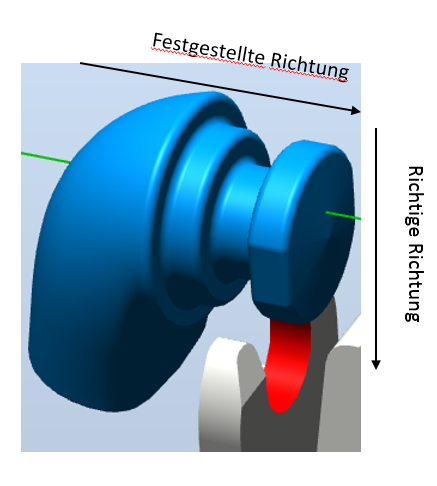
\includegraphics[width=0.3\linewidth]{notclosedarea.png}
				\caption{Ein Beispiel für nicht geschlossenen einschub-relevanten Bereich}
			\end{figure}
			Wie obere Abbildung gezeigt, die Einschubrichtung wird normalerweise auf diesem Fall durch die Achse von Kegel- oder Zylinderoberfläche festgelegt. Aber die richtige Richtung ist anders.
			\item 
			Das Profil des Einschubkörpers und des Festkörpers im einschub-relevanten Bereich kann unter den meisten Umständen übereinstimmen.\\
				\begin{figure}[h!]
				\centering
				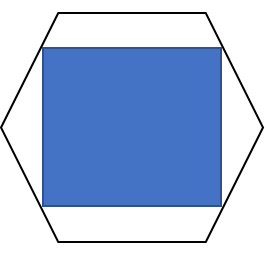
\includegraphics[width=0.3\linewidth]{differentprofile.png}
				\caption{Ein Schnittansicht von einschub-relevanten Bereich}
				\end{figure} 
			Wie untere Abbildung gezeigt, die tatsächlich Berührungsbereich von beiden Körpern besteht nur aus Kanten und keine Flächen. 
			\item Die beiden Körpern müssen als starrer Körper betrachtet werden, d.h. beim Einschubprozess es keine Deformation gibt und das Einrasten ist auch nicht erlaubt. 
			\begin{figure}[h!]
				\centering
				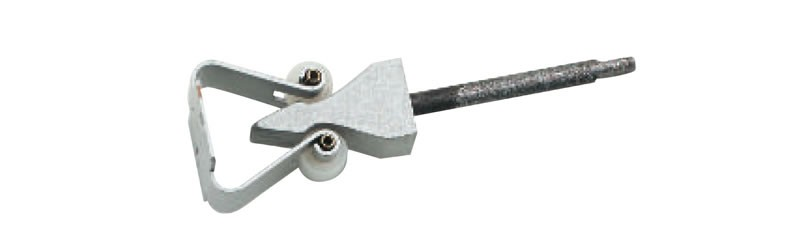
\includegraphics[width=0.5\linewidth]{einrasten.png}
				\caption{Ein Beispiel für das Einrasten}
			\end{figure}
		\end{itemize}
		\textbf{Ergebnisse für einige CAD-Modelle}
			\begin{figure}[b!]
				\centering
				\begin{subfigure}{0.3\linewidth}
					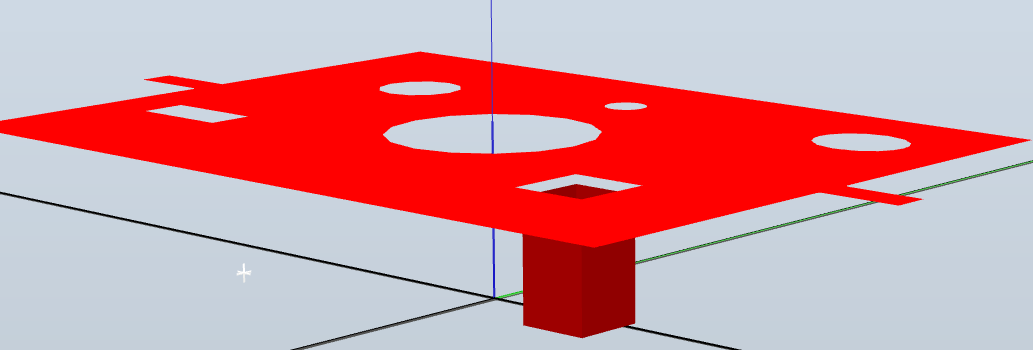
\includegraphics[width=\linewidth]{basefaces1.png}
					\caption{Die gefundene Flächen in Festkörper}
				\end{subfigure}
				\begin{subfigure}{0.3\linewidth}
					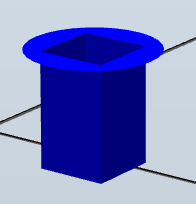
\includegraphics[width=\linewidth]{insertfaces1.png}
					\caption{Die gefundene Flächen in Einschubkörper}
				\end{subfigure}	
				\begin{subfigure}{0.3\linewidth}
					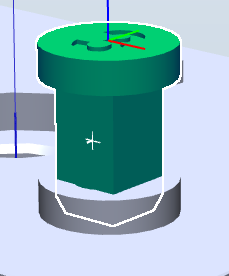
\includegraphics[width=\linewidth]{result1.png}
					\caption{Die gefundene Endposition}
				\end{subfigure}
			\caption{Das erste Ergebnis für Festlegung des Einschubprozesses}
			\end{figure}
			\begin{figure}[h!]
			\centering
			\begin{subfigure}{0.3\linewidth}
				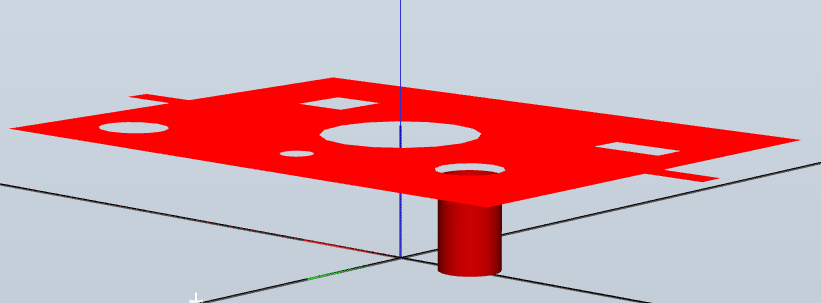
\includegraphics[width=\linewidth]{basefaces4.png}
				\caption{Die gefundene Flächen in Festkörper}
			\end{subfigure}
			\begin{subfigure}{0.3\linewidth}
				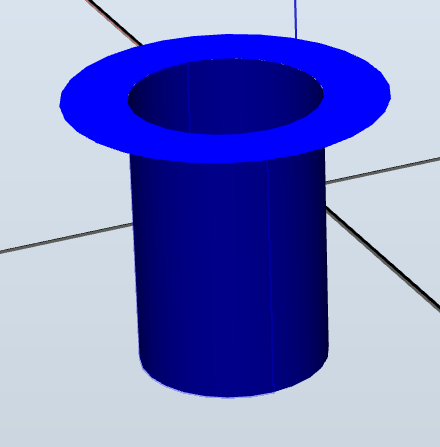
\includegraphics[width=\linewidth]{insertfaces4.png}
				\caption{Die gefundene Flächen in Einschubkörper}
			\end{subfigure}	
			\begin{subfigure}{0.3\linewidth}
				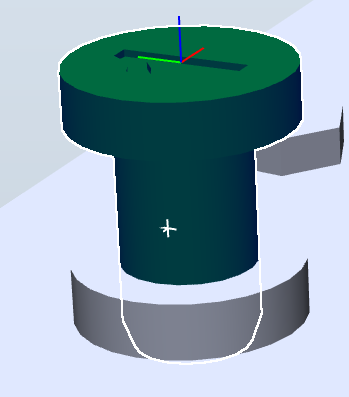
\includegraphics[width=\linewidth]{result4.png}
				\caption{Die gefundene Endposition}
			\end{subfigure}
			\caption{Das zweite Ergebnis für Festlegung des Einschubprozesses}
		\end{figure}
			\begin{figure}[t!]
			\centering
			\begin{subfigure}{0.3\linewidth}
				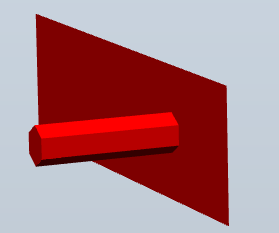
\includegraphics[width=\linewidth]{basefaces2.png}
				\caption{Die gefundene Flächen in Festkörper}
			\end{subfigure}
			\begin{subfigure}{0.3\linewidth}
				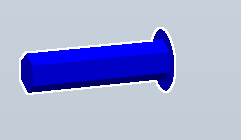
\includegraphics[width=\linewidth]{insertfaces2.png}
				\caption{Die gefundene Flächen in Einschubkörper}
			\end{subfigure}	
			\begin{subfigure}{0.3\linewidth}
				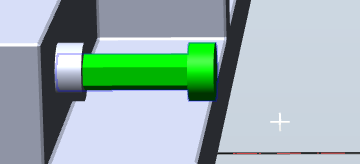
\includegraphics[width=\linewidth]{result2.png}
				\caption{Die gefundene Endposition}
			\end{subfigure}
			\caption{Das dritte Ergebnis für Festlegung des Einschubprozesses}
		\end{figure}
		\begin{figure}[t!]
			\centering
			\begin{subfigure}{0.3\linewidth}
				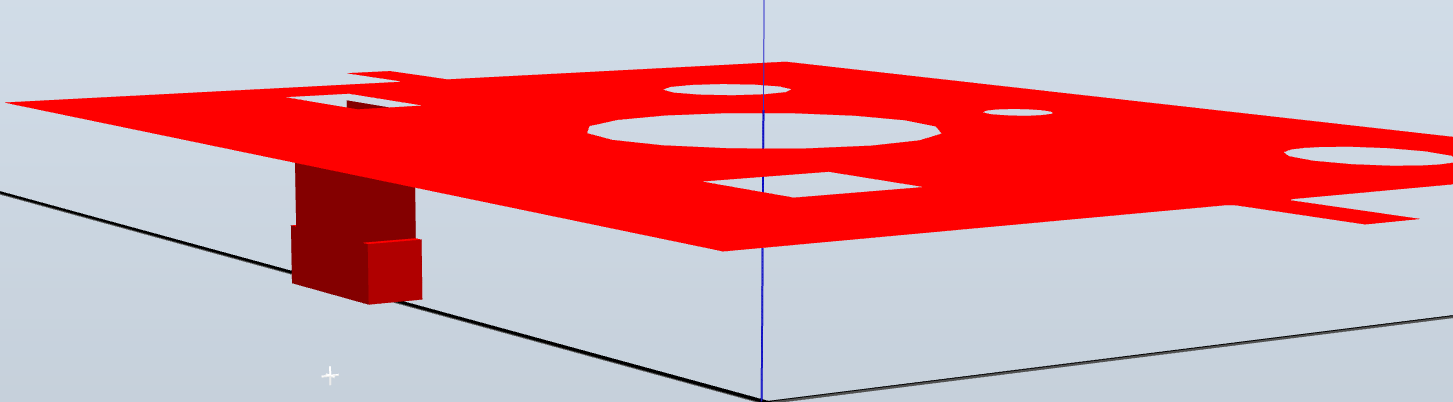
\includegraphics[width=\linewidth]{basefaces3.png}
				\caption{Die gefundene Flächen in Festkörper}
			\end{subfigure}
			\begin{subfigure}{0.3\linewidth}
				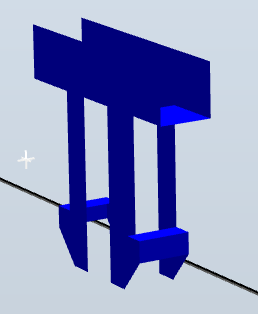
\includegraphics[width=\linewidth]{insertfaces3.png}
				\caption{Die gefundene Flächen in Einschubkörper}
			\end{subfigure}	
			\begin{subfigure}{0.3\linewidth}
				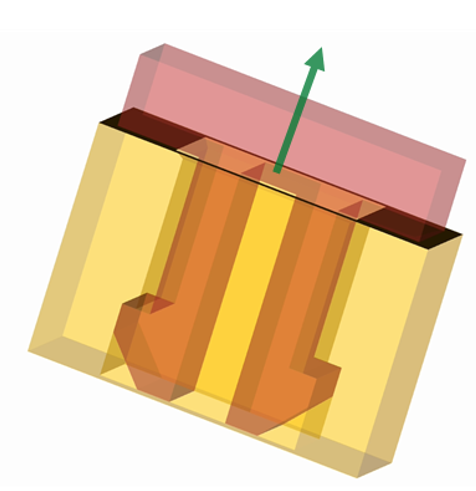
\includegraphics[width=\linewidth]{result3.png}
				\caption{Keine gefundene Endposition wegen Einrasten}
			\end{subfigure}
			\caption{Das vierte Ergebnis für Festlegung des Einschubprozesses}
		\end{figure}
	\hfill
	\pagebreak[6]
	\section{Zusammenfassung}
		In den meisten Fällen kann mithilfe des Algorithmus die erwünschte Einschubrichtung und -distanz festlegen und richtige Informationen für den nächsten Schritt nämlich die automatische Generierung von Roboterprogrammierung erfassen. Wegen der Komplexität von Einschubarten und der Toleranzunterschied von CAD-Modellen kann der Algorithmus auf einige Fälle nicht die richtige Einschubrichtung finden und das Problem ist wie die Einschubrichtung in gewählten Flächen extrahieren soll, sodass die richtige Richtung nicht übersehen werden kann. 
		\bigbreak
		Durch meine Praktikumsarbeit habe ich die Geometrie und Topologie in Computer Grafik besser verstanden und bei Implementierung des Algorithmus habe ich auch RobotStudio und ACIS API vertraut gemacht. Die automtaische Festlegung des Einschubprozesses kann als Ansatz für weitere ähnliche Arbeit für die Automatisierung des Montageprozesses betrachtet werden.
	\pagebreak
	\begin{thebibliography}{1}
		\bibitem{offline-programming} 
		\href{https://en.wikipedia.org/wiki/Off-line_programming_(robotics)}{wikipedia:Off-line programming (robotics)}
		
		\bibitem{robotstudio}
		\href{https://new.abb.com/products/robotics/de/robotstudio}{ABB:Offline-Programmierung leicht gemacht!}
		
		\bibitem{geometrie}
		\href{https://de.wikipedia.org/wiki/Geometrie}{wikipedia:geometrie}
	
		
		\bibitem{topologie}
		\href{https://de.wikipedia.org/wiki/Geodaten#Topologie}{wikipedia:Geodaten}
		
		\bibitem{b-rep}
		\href{https://en.wikipedia.org/wiki/Boundary_representation}{wikipedia: boundary representation}
		
		\bibitem{kurve}
		\href{https://de.wikipedia.org/wiki/Kurve_(Mathematik)}{wikipedia: Kurve (Mathematik)}
		
		\bibitem{cli}
		\href{https://de.wikipedia.org/wiki/C%2B%2B/CLI}{wikipedia: C++/CLI}
	\end{thebibliography}
	\pagebreak
	\listoffigures
	\pagebreak
	\section*{Abkürzungsverzeichnis}
	\begin{acronym}[OLP]
		\acro{olp}[OLP]{Offline-Programmierung}
	\end{acronym}
	\begin{acronym}[TCP]
		\acro{tcp}[TCP]{Werkzeugarbeitspunkt}
	\end{acronym}
	\begin{acronym}[SDK]
		\acro{sdk}[SDK]{Software Development Kit}
	\end{acronym}
	\begin{acronym}[b-rep]
		\acro{b-rep}[b-rep]{boundary representation}
	\end{acronym}
	\begin{acronym}[step]
		\acro{step}[STEP]{the Standard for the Exchange of Product Model data}
	\end{acronym}
	\begin{acronym}[gui]
		\acro{gui}[GUI]{grafische Benutzeroberfläche}
	\end{acronym}
	\begin{acronym}[acis]
		\acro{acis}[ACIS]{3D ACIS Modeler}
	\end{acronym}
	\begin{acronym}[api]
		\acro{api}[API]{application programm interface}
	\end{acronym}
	\begin{acronym}[cli]
		\acro{cli}[CLI]{common language infrastructure}
	\end{acronym}
	\begin{acronym}[cil]
		\acro{cil}[CIL]{common intermediate language}
	\end{acronym}
	\begin{acronym}[gc]
		\acro{gc}[GC]{garbage collection}
	\end{acronym}

\end{document}